\section{Introduction}
\begin{frame}{}
  \LARGE RNNs : \textbf{Introduction}
\end{frame}

% Slide 7: Traditional Language Models
\begin{frame}{Traditional Language Models}
  \centering
  
\includegraphics[width=0.9\paperwidth,height=0.95\paperheight,keepaspectratio]{assets/Lecture-3_Recurrent_Neural_Networks/slide_006.png}
\end{frame}

% Slide 8: N-grams
\begin{frame}{N-grams}
  \begin{itemize}
      \item Bigrams: $P(w_{2}|w_{1})=\frac{count(w_{1},w_{2})}{count(w_{1})}$
      \item Trigrams: $P(w_{3}|w_{1},w_{2})=\frac{count(w_{1},w_{2},w_{3})}{count(w_{1},w_{2})}$
      \item $P(w_{1},w_{2},w_{3})=P(w_{1})\times P(w_{2}|w_{1})\times P(w_{3}|w_{2})$
      \item \textbf{Limitations:} Large N-grams need significant space and RAM.
  \end{itemize}
\end{frame}

% Slide 9: N-grams - Limitations

\begin{frame}{N-grams: Limitations}
  \begin{itemize}
      \item N-gram tables consume a lot of memory.
      \item \textbf{Fixed context window:} only the previous $(n-1)$ words are conditioned on.
      \item \textbf{Data sparsity:} larger $n$ implies exponentially many $n$-grams; many combinations are rare or unseen in training data.
      \item \textbf{No learning or adaptability:} counts and normalization only---not learned representations in the neural sense.
      \item Different types of \textbf{RNNs} are the \textbf{preferred alternative}.
  \end{itemize}
\end{frame}

% Slide 10: What is an RNN?
\begin{frame}{What is an RNN?}
  A neural network with loops allowing information to persist.
  \textbf{Core Elements:}   
  \begin{itemize}
      \item Hidden State $h_{t}$ captures memory of previous inputs.
      \item Input $X_{t}$, Output $y_{t}$.
      \item Parameter sharing: Same weights used across time steps.
  \end{itemize}
  \textbf{Mathematical Formulation:}
  \begin{itemize}
      \item $h_{t}=tanh(W_{hh}h_{t-1}+W_{xh}x_{t}+b_{h})$
      \item $y_{t}=W_{hy}h_{t}+b_{y}$
  \end{itemize}
  \textbf{This recurrence allows information to propagate through time.}
\end{frame}

% Slide 11: Why Use RNNs?
\begin{frame}{Why Use RNNs?}
  \begin{itemize}
      \item RNNs target \textbf{sequential data} where order matters (language, time series, speech).
      \item \textbf{Capturing context:} a hidden state carries information from previous steps.
      \item Example: word meaning often depends on preceding words; RNNs model such dependency.
      \item \textbf{Variable-length inputs} within a single architecture.
      \item \textbf{Temporal patterns} in language modeling, speech, financial series, etc.
  \end{itemize}
\end{frame}

% Slide 12: Why Use RNNs?
\begin{frame}[Why Use RNNs]
  \centering
  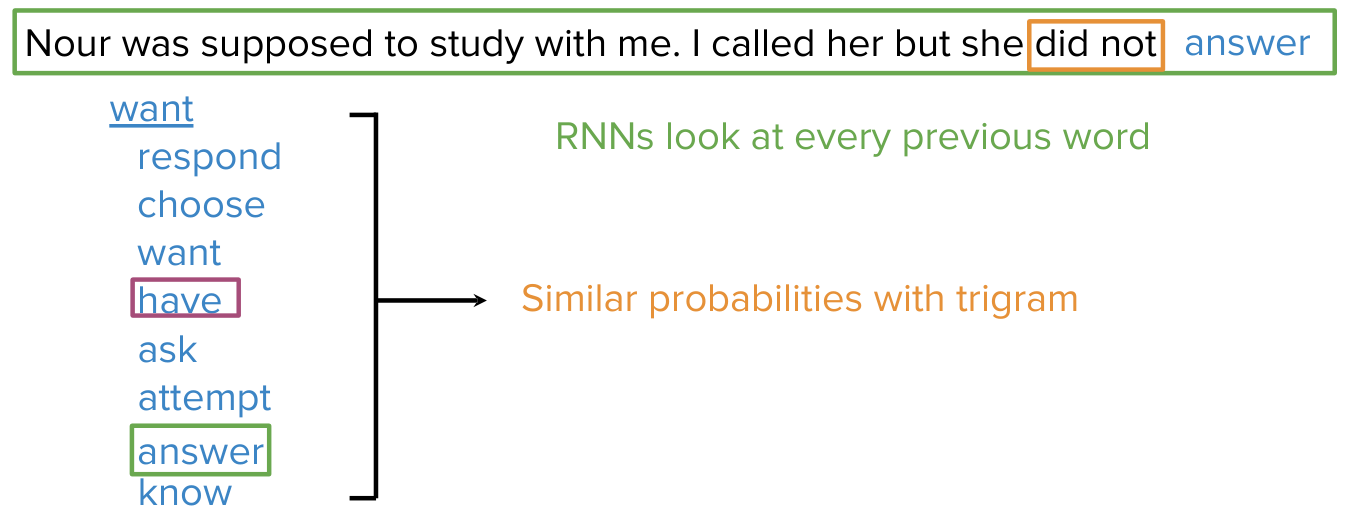
\includegraphics[width=0.9\paperwidth,height=0.95\paperheight,keepaspectratio]{assets/Lecture-3_Recurrent_Neural_Networks/pdf_page_012.png}
\end{frame}

% Slide 13: RNNs Basic Structure
\begin{frame}{RNNs Basic Structure}
  \centering
  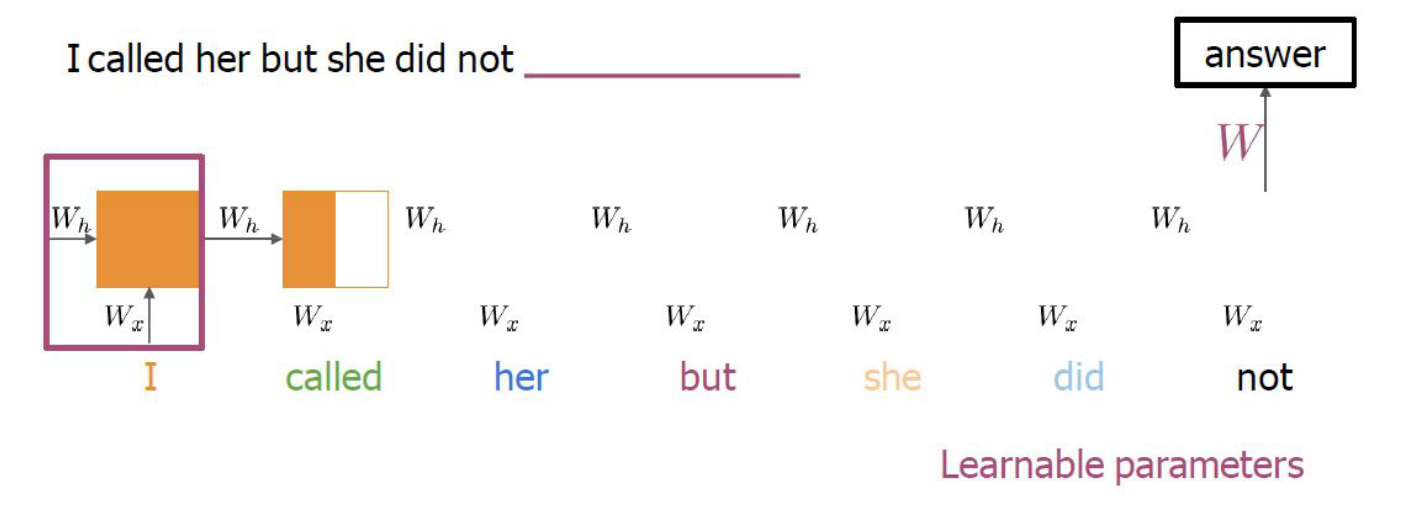
\includegraphics[width=0.9\paperwidth,height=0.95\paperheight,keepaspectratio]{assets/Lecture-3_Recurrent_Neural_Networks/slide_011.png}
\end{frame}
